
\documentclass[paper=a4, fontsize=11pt]{scrartcl} % A4 paper and 11pt font size

\usepackage[T1]{fontenc} % Use 8-bit encoding that has 256 glyphs
\usepackage[english]{babel} % English language/hyphenation
\usepackage{amsmath,amsfonts,amsthm} % Math packages
\usepackage{cite}
\usepackage{graphicx}
%\usepackage{algorithm} % algorithm package


\usepackage{sectsty} % Allows customizing section commands
\allsectionsfont{\centering \normalfont\scshape} % Make all sections centered, the default font and small caps

\usepackage{fancyhdr} % Custom headers and footers
\pagestyle{fancyplain} % Makes all pages in the document conform to the custom headers and footers
\fancyhead{} % No page header - if you want one, create it in the same way as the footers below
\fancyfoot[L]{} % Empty left footer
\fancyfoot[C]{} % Empty center footer
\fancyfoot[R]{\thepage} % Page numbering for right footer
\renewcommand{\headrulewidth}{0pt} % Remove header underlines
\renewcommand{\footrulewidth}{0pt} % Remove footer underlines
\setlength{\headheight}{13.6pt} % Customize the height of the header

%%%%%%%%%%%%%%%%%%%%%%%%%%%%%%%%%%%%%%%%%%%%%
\DeclareMathOperator*{\argmin}{arg\,min}
\newtheorem{theorem}{Theorem}[section]
\newtheorem{lemma}[theorem]{Lemma}
\newtheorem{proposition}[theorem]{Proposition}
\newtheorem{corollary}[theorem]{Corollary}
%%%%%%%%%%%%%%%%%%%%%%%%%%%%%%%%5
\numberwithin{equation}{section} % Number equations within sections (i.e. 1.1, 1.2, 2.1, 2.2 instead of 1, 2, 3, 4)
\numberwithin{figure}{section} % Number figures within sections (i.e. 1.1, 1.2, 2.1, 2.2 instead of 1, 2, 3, 4)
\numberwithin{table}{section} % Number tables within sections (i.e. 1.1, 1.2, 2.1, 2.2 instead of 1, 2, 3, 4)

\setlength\parindent{0pt} % Removes all indentation from paragraphs - comment this line for an assignment with lots of text





%----------------------------------------------------------------------------------------
% new commands
%----------------------------------------------------------------------------------------
\newcommand{\der}{\text{d}}
\newcommand{\coder}[1]{\texttt{#1}}


\title{HPC Project Summary}
\author{Yair Daon}
\date{}

\pdfinfo{%
  /Title    ()
  /Author   (Yair Daon)
  /Creator  ()
  /Producer ()
  /Subject  ()
  /Keywords ()
}

\begin{document}
\maketitle
\begin{abstract}
I solve scalar advection equation using OpenCl on GPUs and create visualizations.
\end{abstract}
\section{Problem statement}
Consider the followin PDE:
Consider $\frac{\partial T}{\partial t} + \sum_{i=1}^{d} \frac{\partial u^{(i)}T}{\partial x^{(i)}} = 0$.
$T$ is a tracer - ``a drop of ink in water'', $d$ is the dimension. Focus on flows such that $\sum_{i=1}^{d} \frac{\partial u^{(i)}}{\partial x^{(i)}} = 0$ - incompressible.
We'd like to solve this equation numerically and simulate the results.



\section{Solution Methodology - numerics}
Consider the 2D case. We follow \cite{terrorist}. 
Use finite volume and then a RK method. Here we consider $d=2$. First, partition spatial domain to boxes. Denote centers by $(x_j, y_k)$.
Integrate the equation in all coordinates over box.  This gives integrals like 
$\int_{x_i - \frac{\Delta x}{2}}^{x_i + \frac{\Delta x}{2}} F(x,y_j) dx$. We estimate these by
the value at the center - $\int_{x_i - \frac{\Delta x}{2}}^{x_i + \frac{\Delta x}{2}} F(x,y_j) dx \approx F(x_i ,y_j)\Delta x$.
Finally, when the dust settles, 
  $$
  \frac{\der T_{ij}}{\der t} = -\frac{uT(x_{i+\frac{1}{2}} , y_j) - uT(x_{i-\frac{1}{2}} , y_j)}{\Delta x} -\frac{vT(x_i , y_{j+\frac{1}{2}}) - vT(x_i , y_{j-\frac{1}{2}})}{\Delta y}.
$$
with $uT(x_{i+\frac{1}{2}} , y_j)= u(x_i + \frac{\Delta x}{2},y_j) \frac{T_{ij} + T_{i+1,j}}{2}$ etc. - we estimate $T$ on cell edges as 
an average of the two neighbouring cells. This procedure results in an ODE of the form $\frac{\der T}{\der t} = AT$, with $A$ linear in $T$. We solve this
via a Runge Kutta method.

\section{Solution Methodology - computing}

\subsection{PyOpenCl}
For accessing OpenCl devices, I used PyOpenCl \cite{pyopencl}. This is a wonderful python package written by Andreas Kl\"ockner. 
It makes creating visualizations and initial conditions a whole lot easier, not to 
mention freeing memory and all the nice things python does seamlessly. It is important to note that PyOpenCl handles the host side. 
The device (GPU in my case) still runs a native OpenCl code which is 
compiled just in time.

\subsection{Mathematica} 
If we do a n\"aive RK, we'd have to
send data back and forth between main memory and the GPU. Recalling the rule of thumb that says 
\\
\\
\centerline{\Large{``Flops are cheap, memory access is expensive``}}
\\

 it's clear that one has to calculate the new $T_{ij}$ locally as a function of old local values $T_{ij}, T_{i,(j+1)}$ etc. 
 Deriving the required equations manually is a horrible task, so I turned to Mathematica \cite{math}. It is a high level and abstract
programming language suitable for symbolic manipulations. 
Hence, I define the following operator in Mathematica (for 2D flows. 3D is similar):

\begin{verbatim}
A = Function[T , Function[{arr,i,j},  
			  -(u[i+0.5,j]*( T[arr,i+1,j  ] + T[arr,i,j] ) - 
			  u[i-0.5 ,j]*(T[arr,i,j] +T[arr,i-1,j  ] ))/(2*HX)  
			  -(v[i,j+0.5]*( T[arr,i  ,j+1] + T[arr,i,j] ) - 
			  v[i ,j-0.5]*(T[arr,i,j] +T[arr,i  ,j-1] ))/(2*HY)
 				]]
\end{verbatim}
where \coder{Function} takes the role of $\lambda$ in $\lambda$ calculus.
I use it to get the RK step explicitly. For example, the expression for the 
new $T_{ij}$ is found via the following RK mehtod:
\begin{verbatim}
  rk3     = T[Tin,i,j] - HT*A[T][Tin,i,j] - 0.5*HT*HT*A[A[T]][Tin,i,j] +
                         0.25*HT*HT*HT*A[A[A[T]]][Tin,i,j]
  rk3     = ToString[CForm[Simplify[rk3]]]
\end{verbatim}

This allows me to let Mathematica derive any order of RK method I want, owing to the linearity of the operator A. 
As an example, I paste in the appendix the C code the above script generates (after some minor string modifications) for a
second order RK method in 2D. 
The advantage is a huge save in memory transfer between the host and the device. As a bonus, generalization to higher
dimensions (i.e. 3) is trivial (add indices and copy-paste).

\subsection{Inlining constants and the Kernel}
Since I was using python, I allowed myself to add all the parameters as constatns (by using \coder{\#define PI 3.14159...} etc. This 
might have saved some communication and some flops, but is just a tiny bonus python allows to use. The main advantage python gave me
in this respect, is the ability to write a ''generic`` kernel and just substitute, on the fly, the correct expression for the RK step.
This makes debugging easy and automate the process of performing simulations considerably.


\subsection{Machines}
I used my CIMS machine's CPU and GPU and also used the Tahiti and Cedar GPU processors on opencl3.



\section{Performance}
At first I was amazed at how fast the code runs. There are considerable differences in speed between a third and a second order RK methods.
The code shows beautiful weak scalability.

\begin{figure}[ht!]
\centering
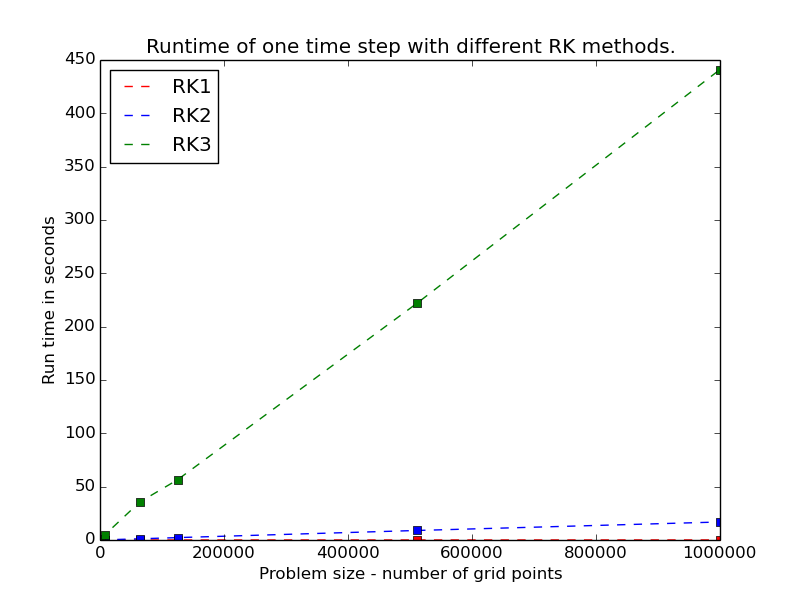
\includegraphics[width=90mm]{3d.png}
\caption{Weak scalability of time of a RK steps \label{overflow}}
\end{figure}

\section{What have I gained}
I got exprerience with using OpenCl, through PyOpenCl (which made deebugging and visualization much easier). I believe that writing 
computational code in lower level language (here, OpenCL) and using an interface from a higher level language (PyOpenCl) is good
practice when doing scientific computing. This is mainly because there is usually a small chunk of code that does the numerics (this has to 
run FAST) and other bits that can be made slower, making the programmer's life a whole lot easier.

I also learned that every vendor has their own nuiances and so fitting your code to the machine it will run on isn't necessarily
a bad idea. My problem was creating code that is portable between Intel and AMD - the errors they give are not consistent.

I leanred to use Mathematica for deriving complicated expressions. The main (only?) idea was to use $\lambda$ calculus
and treat arrays as functions and indices as their variables. This will surely prove useful any time I want to perform a numeric
simulation that relies on discretizations.

I also go familiar with some fluid dynamics, which is cool.

\section{What I did not do and failures}
I did not make a 3D visualization, lacking an appropriate flow problem. I did not cache the input array to local memory on the OpenCl device, which 
could have sped things up. However, the code ran so fast that I did not feel a need to do so.

\bibliographystyle{unsrt}

\bibliography{refs}

\newpage

\section{Appendix}
Here is the C code Mathematica spits out for a 2D 2nd order Runge Kutta method. For higher orders and dimensions, it looks even worst.
This is the main reason I had to use a symbolic package.
\begin{verbatim}
T(Tin,xCol,yRow) + HT*(-(-((T(Tin,-1 + xCol,yRow) + T(Tin,xCol,yRow))*u(-0.5 + 
xCol,yRow))+ (T(Tin,xCol,yRow) + T(Tin,1 + xCol,yRow))*u(0.5 + xCol,yRow))/(2.
*HX) - (-((T(Tin,xCol,-1 + yRow) + T(Tin,xCol,yRow))*v(xCol,-0.5 + yRow)) + (T
(Tin,xCol,yRow) + T(Tin,xCol,1 + yRow))*v(xCol,0.5 + yRow))/(2.*HY)) - (0.125*
HT*HT*(HX*(v(xCol,-0.5 + yRow)*(-(HY*T(Tin,-1 + xCol,-1 + yRow)*u(-0.5 + xCol,
-1 + yRow)) - HY*T(Tin,-1 + xCol,yRow)*u(-0.5 + xCol,yRow) - HY*T(Tin,xCol,yRow
)*u(-0.5 + xCol,yRow) + HY*T(Tin,1 + xCol,-1 + yRow)*u(0.5 + xCol,-1 + yRow) + 
HY*T(Tin,xCol,yRow)*u(0.5 + xCol,yRow) + HY*T(Tin,1 + xCol,yRow)*u(0.5 + xCol
,yRow) - HX*T(Tin,xCol,-2 + yRow)*v(xCol,-1.5 + yRow) - T(Tin,xCol,-1 + yRow)
*(HY*u(-0.5 + xCol,-1 + yRow) - HY*u(0.5 + xCol,-1 + yRow) + HX*v(xCol,-1.5 +
yRow)) + HX*T(Tin,xCol,yRow)*v(xCol,0.5 + yRow) + HX*T(Tin,xCol,1 + yRow)*v(xCol
,0.5 + yRow)) + v(xCol,0.5 + yRow)*(HY*T(Tin,-1 + xCol,yRow)*u(-0.5 + xCol,yRow) 
+ HY*T(Tin,-1 + xCol,1 + yRow)*u(-0.5 + xCol,1 + yRow) + HY*T(Tin,xCol,1 + yRow)
*u(-0.5 + xCol,1 + yRow) - HY*T(Tin,1 + xCol,yRow)*u(0.5 + xCol,yRow) - HY*T(Tin
,xCol,1 + yRow)*u(0.5 + xCol,1 + yRow) - HY*T(Tin,1 + xCol,1 + yRow)*u(0.5 + xCol
,1 + yRow) + HX*T(Tin,xCol,-1 + yRow)*v(xCol,-0.5 + yRow) + T(Tin,xCol,yRow)*(HY*
u(-0.5 + xCol,yRow) - HY*u(0.5 + xCol,yRow) + HX*v(xCol,-0.5 + yRow)) - HX*T(Tin,
xCol,1 + yRow)*v(xCol,1.5 + yRow) - HX*T(Tin,xCol,2 + yRow)*v(xCol,1.5 + yRow)))
+ HY*(-(u(-0.5 + xCol,yRow)*(HY*T(Tin,-2 + xCol,yRow)*u(-1.5 + xCol,yRow) - HY*T
(Tin,xCol,yRow)*u(0.5 + xCol,yRow) - HY*T(Tin,1 + xCol,yRow)*u(0.5 + xCol,yRow) + 
HX*T(Tin,-1 + xCol,-1 + yRow)*v(-1 + xCol,-0.5 + yRow) - HX*T(Tin,-1 + xCol,1 + 
yRow)*v(-1 + xCol,0.5 + yRow) + T(Tin,-1 + xCol,yRow)*(HY*u(-1.5 + xCol,yRow) +
HX*v(-1 + xCol,-0.5 + yRow) - HX*v(-1 + xCol,0.5 + yRow)) + HX*T(Tin,xCol,-1 + 
yRow)*v(xCol,-0.5 + yRow) + HX*T(Tin,xCol,yRow)*v(xCol,-0.5 + yRow) - HX*T(Tin,
xCol,yRow)*v(xCol,0.5 + yRow) - HX*T(Tin,xCol,1 + yRow)*v(xCol,0.5 + yRow))) +
u(0.5 + xCol,yRow)*(HY*T(Tin,-1 + xCol,yRow)*u(-0.5 + xCol,yRow) - HY*T(Tin,1 + 
xCol,yRow)*u(1.5 + xCol,yRow) - HY*T(Tin,2 + xCol,yRow)*u(1.5 + xCol,yRow) + HX*
T(Tin,xCol,-1 + yRow)*v(xCol,-0.5 + yRow) - HX*T(Tin,xCol,1 + yRow)*v(xCol,0.5 +
yRow) + T(Tin,xCol,yRow)*(HY*u(-0.5 + xCol,yRow) + HX*v(xCol,-0.5 + yRow) - HX*v
(xCol,0.5 + yRow)) + HX*T(Tin,1 + xCol,-1 + yRow)*v(1 + xCol,-0.5 + yRow) + HX*T
(Tin,1 + xCol,yRow)*v(1 + xCol,-0.5 + yRow) - HX*T(Tin,1 + xCol,yRow)*v(1 + xCol
,0.5 + yRow) - HX*T(Tin,1 + xCol,1 + yRow)*v(1 + xCol,0.5 + yRow)))))/(HX*HX*HY*HY)
\end{verbatim}


\end{document}
